
\FloatBarrier

\section{Система Ван-дер-Поля} %  % {{{1 _VDP_
\label{atu:sect:vdp}

\LinkRef{
  vdp: ASAU-16, 17(alt), ITMM-2011
}

\subsection{Визначення системи та аналіз її динаміки} %{{{2 vdp_task

Модель нелінійної автоколивальній системи
Ван-Дер-Поля~(\ref{atu:eq:vdp}) широко використовується при дослідженні
динаміки коливальних систем, в яких відбувається поповнення
енергії системи з зовнішнього джерела~\cite{Ginoux2012VanDP,anisch_nonlin_eff,magni_theory_dyn_chaos,atu_asau16,atu_st75,chulichkcov_mm_ml_dyn}:
%
\begin{equation}
 \ddot{x} - \varepsilon (1-x^2)  \dot{x} + \Omega_0^2 x  = u(t) .
\label{atu:eq:vdp}
\end{equation}
\noindent
де
\(x(t)\) --- координата коливань,
\(\varepsilon \) --- параметр, що визначає отримання енергії системою,
\(\Omega_0 \) --- власна частота при \(\varepsilon= 0 \),
\( u (t) \) --- зовнішнє вплив, що збурює.

При \(\varepsilon> 0 \) і \(u (t) = 0 \) розглянута система реалізує режим
автоколивань з постійною частотою, яка залежить від \(\varepsilon \):
%
\begin{equation}
\Omega \approx \Omega_0 \sqrt{ 1 - \left( \frac{\varepsilon}{2 \Omega_0} \right)^2 }.
\label{atu:eq:vdp_Omega}
\end{equation}

При цьому амплітуда коливань залишається майже незмінною, а
сама форма коливань приймає все більш нелінійний характер.

Під впливом вхідного гармонійного сигналу
\( u(t) = U_{in} \sin ( \omega_{in} t ) \)
система~(\ref{atu:eq:vdp}) може проявляти регулярну, складно-періодичну
і хаотичну динаміку~\cite{atu_itcs2011,atu_ISDMCI2011,gang_chaos_on_phase_noise,baranov_chaos_vdp,kuznetsov_phenomen_vdp,math5040070}.

Ідентифікований параметр \(\varepsilon \) характеризує надходження
енергії у систему. При
$ x \approx 0 $ членом з
$ x ^ 2 $ можна знехтувати, і нелінійність вироджується в ``негативне тертя''.
При великих амплітудах коливань член з
$x^2$ починає переважати, там самим обмежуючи зростання
амплітуди. Існує також система, яка має назву
Ван-дер-Поля-Дуффінга~\cite{landa_nonlin_vivro_waves}, та об'єднує властивості
даної системи і системи Дуффінга.

При аналізі чисельного моделювання системи~(\ref{atu:eq:vdp})
слід обережно ставиться до висновків про тип динаміки, які
можна зробити, виходячи з фазового або розширеного фазового
портрета.
Наприклад, на рис.~\ref{atu:f:vdp_phase_f_reg}, за умов
$ \varepsilon = 1.50 $,
$ U_{in} = 0.3 $,
$ \omega_{in} = 0.27 $ на лівому графіку фазова траєкторія виходить
щільною, однак спектр свідчить про регулярну динаміку з
обмеженим набором частот.

\begin{figure}[ht!]
\begin{center}
  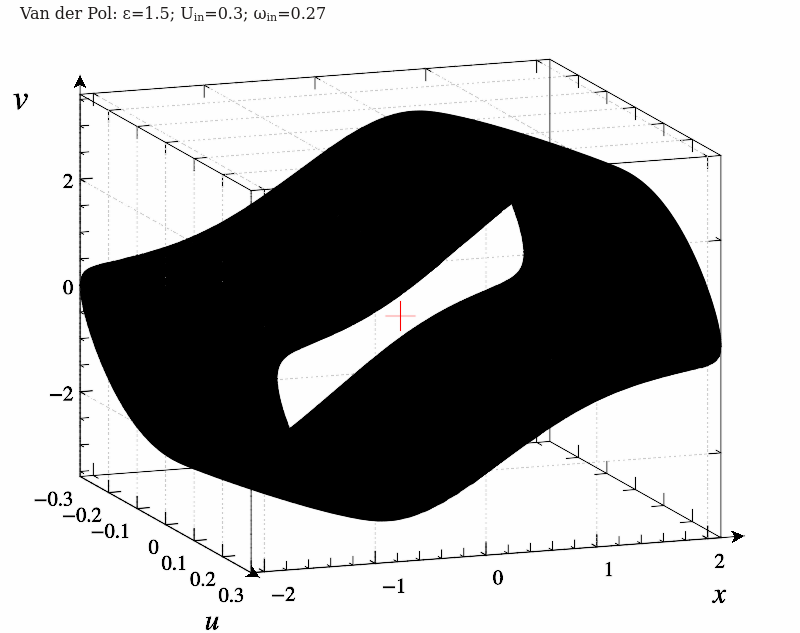
\includegraphics[width=0.49\textwidth]{p/cha/vdp/vdp_0-p_ph2d_1x50_0x30_0x27.png}
  \hfill
  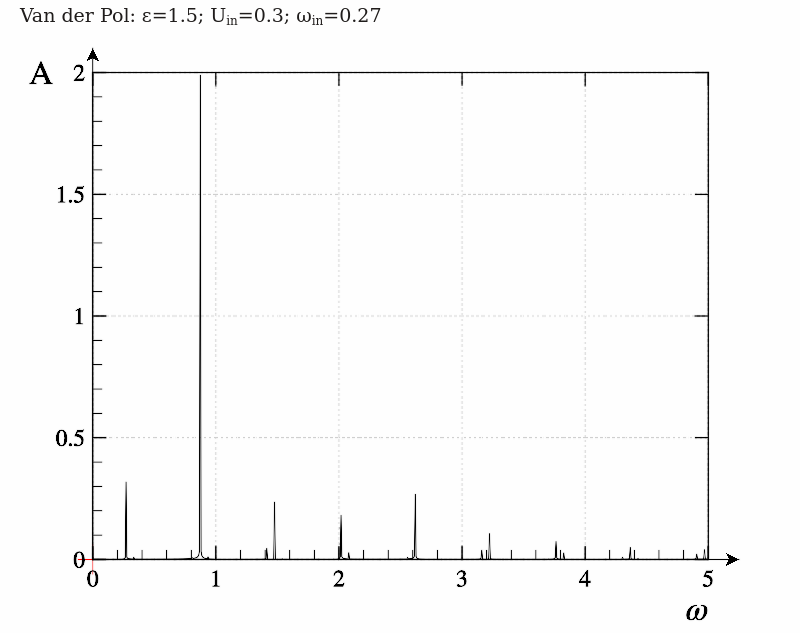
\includegraphics[width=0.49\textwidth]{p/cha/vdp/vdp_fft-p_f_1x50_0x30_0x27.png}
\end{center}
\caption{Розширений фазовий портрет і спектр системи Ван-дер-Поля (\ref{atu:eq:vdp}) в режимі регулярних коливань}
\label{atu:f:vdp_phase_f_reg}
\end{figure}

Безпосередньо хаотичні коливання цієї системи часто
характеризуються менш вираженою щільністю аттрактора. Проте,
ділянки складного спектра (рис.~\ref{atu:f:vdp_phase_f_chaos}) свідчать на
користь хаосу. Дана ілюстрація відповідає умовам
$ \varepsilon = 2.65 $,
$ U_{in} = 1.2 $,
$ \omega_{in} = 0.27 $. При цьому малі зміни параметрів, наприклад зниження
величини
$ \varepsilon $ до
$ 2.5 $ призводить до реалізації режиму простих регулярних
коливань.

\begin{figure}[ht!]
\begin{center}
  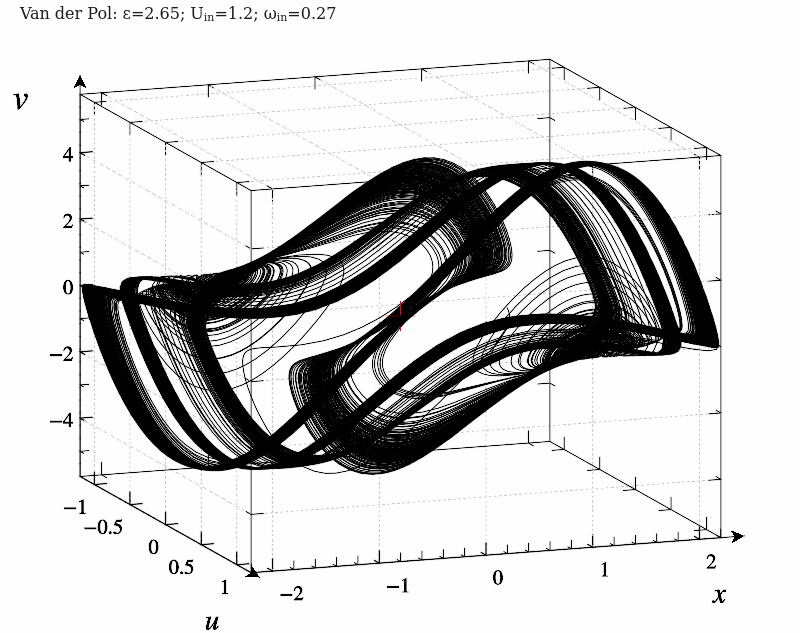
\includegraphics[width=0.49\textwidth]{p/cha/vdp/vdp_0-p_ph2d_2x65_1x20_0x27.png}
  \hfill
  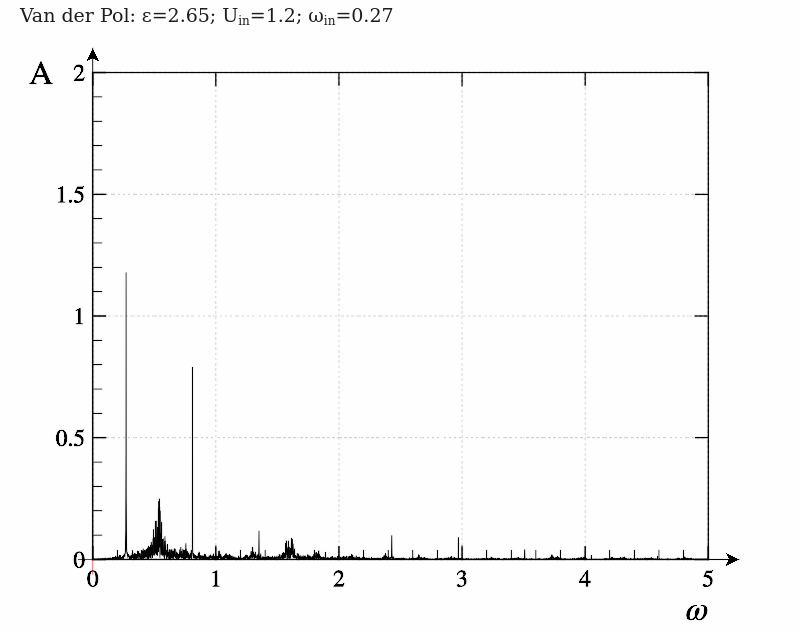
\includegraphics[width=0.49\textwidth]{p/cha/vdp/vdp_fft-p_f_2x65_1x20_0x27.png}
\end{center}
\caption{Розширений фазовий портрет і спектр системи Ван-дер-Поля (\ref{atu:eq:vdp}) в режимі хаотичних коливань}
\label{atu:f:vdp_phase_f_chaos}
\end{figure}

Аналіз спектру системи Ван-дер-Поля, як і багатьох інших систем
динамічного хаосу, слід проводити, враховуючи спектральну
роздільну здатність. Наприклад, на рис.~\ref{atu:f:vdp_phase_f_complex} представлені
результати моделювання системи при
$ \varepsilon = 4.8 $,
$ U_{in} = 0.7 $,
$ \omega_{in} = 0.7 $. В спектрі системи спостерігаються ділянки з дуже
близько розташованими піками. При недостатній роздільної
здатності цю ділянку буде прийнято за зону суцільного
спектру. Це може привести до помилкового висновку про хаотичність системи,
особливо з врахуванням структури аттрактора.

\begin{figure}[ht!]
\begin{center}
  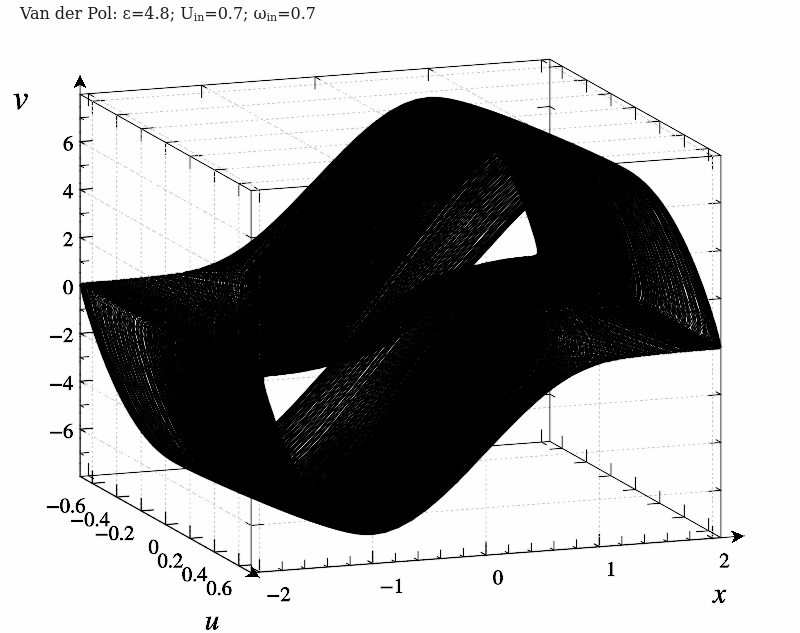
\includegraphics[width=0.49\textwidth]{p/cha/vdp/vdp_0-p_ph2d_4x80_0x70_0x70.png}
  \hfill
  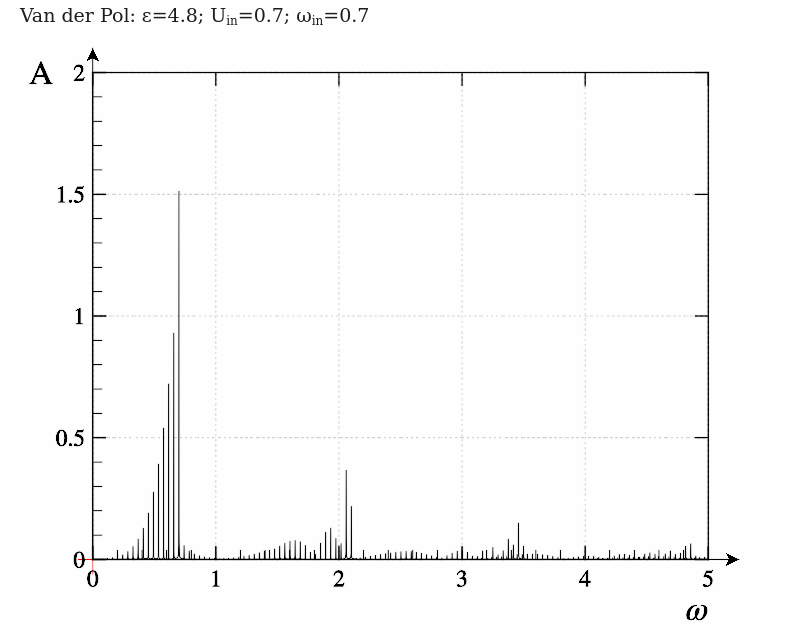
\includegraphics[width=0.49\textwidth]{p/cha/vdp/vdp_fft-p_f_4x80_0x70_0x70.png}
\end{center}
\caption{Розширений фазовий портрет і спектр системи Ван-дер-Поля (\ref{atu:eq:vdp}) в режимі складних регулярних коливань}
\label{atu:f:vdp_phase_f_complex}
\end{figure}

При аналізі фізичних систем немає можливості довільним чином
задавати час вимірювання для отримання спектра з необхідною
роздільною здатністю. Більш того, з урахуванням обмеженої точності вимірів
немає можливості точно визначити показники Ляпунова. Таким
чином, цілком можливе існування систем, які не відрізняються
від хаотичних при проведенні вимірювань, але не є хаотичними в
строгому розумінні. Проте, з точки зору задачі ідентифікації,
цей випадок практично не відрізняється від реального хаосу,
і вимагає застосування відповідних методів і критеріїв.

% }}}2


\subsection{Аналіз і вибір критеріїв}%{{{2

На відміну від систем Лоренца, Ресслера та їм подібних, у системи
Ван-дер-Поля є тільки одна величина, що спостерігається: $x(t)$. Це
відразу сильно обмежує коло критеріїв, які потребують аналізу.

На перший погляд, якщо доступний сигнал
$x(t)$, то можна обчислити сигнали
$\dot{x}(t) $ і
$\ddot{x}(t)$. Після цього, підставивши отримані залежності
в (\ref{atu:eq:vdp}), можна отримати значення ідентифікованого
параметра. Насправді, це можливо тільки в разі практично
повної відсутності перешкод. Навіть невеликий (0.001\%) рівень
помилок вимірювання при обчисленні похідних, особливо другої,
призводить до абсолютно довільним результатам. Таким чином,
для цієї системи без застосування інтегральних критеріїв
немає можливості створити працездатну систему ідентифікації.

Критерії
$q_{x^2} $,
$q_{rx} $ і
$q_{|x|} $ відрізняються для цього завдання не
принципово. Незважаючи на те, що ці величини в даному конкретному
разі не відображають будь-якої закон збереження, їх застосування
може бути виправданим~\cite{atu_asau17}. При зростанні параметра
$ \varepsilon $ система все більше виявляє нелінійні властивості. Це
виражається в тому, що при однаковій амплітуді сигналу
залежність
$x(t)$ більшу частину часу проводить у районі амплітудних
значень, що призводить до зростання цих критеріїв. Для
визначеності в подальшому будемо використовувати
$q_{x^2}$.

Також має сенс розглянути досить очевидний для коливальних
систем критерій
$q_T$, що полягає у вимірюванні ``періоду''~\cite{atu_asau16}. Очевидно, що
поняття періоду для хаотичних систем не можна застосовувати. Однак,
можна прийняти за поточне значення періоду інтервал часу між
двома послідовними спрацьовуваннями коректно налаштованого
тригера Шмідта, на вхід якого подається сигнал
$x(t)$. Цей підхід використовується при побудові вхідних
ланцюгів частотомеров. При цьому автоматично відбувається
усереднення на інтервалах порядку цього ``періоду''. Однак,
для систем ідентифікації таке усереднення швидше за все
буде недостатнім, особливо в хаотичних і складно-періодичних
режимах. Отже, має сенс використовувати додаткове усереднення,
наприклад~(\ref{atu:eq:qlin}).

Розглянемо характерні залежності розглянутих критеріїв,
отримані в результаті моделювання динаміки системи
(\ref{atu:eq:vdp}). На рис.~\ref{atu:f:vdp_q1} представлений вид цих залежностей
для різних умов.


\begin{figure}[ht!]
\begin{center}
  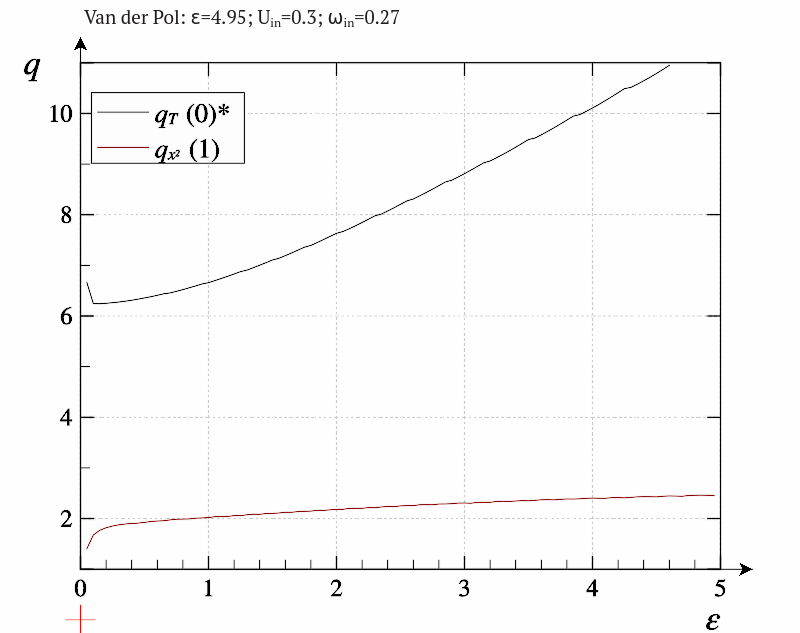
\includegraphics[width=0.49\textwidth]{p/cha/vdp/vdp_q-p_q_0x30_0x27.png}
  \hfill
  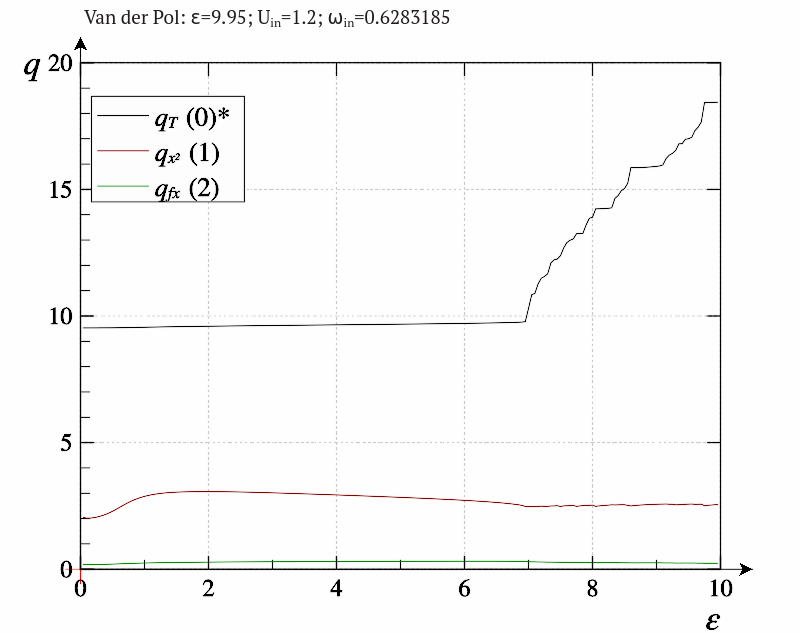
\includegraphics[width=0.49\textwidth]{p/cha/vdp/vdp_q-p_q_1x20_0x6283185.png}
\end{center}
\caption{Залежності $ q_{x ^ 2} (\varepsilon) $ і $ q_T (\varepsilon) $ системи Ван-дер-Поля}
\label{atu:f:vdp_q1}
\end{figure}

Лівий графік відповідає такому набору параметрів, при якому
спостерігається періодичний і складно-періодичний рух. При цьому
обидва критерії підходять для синтезу системи ідентифікації,
а критерій $ q_T $ виявляє меншу нелінійність. Правий графік відображає
випадок, коли зміна параметра
$ \varepsilon $ призводить до істотної зміни поведінки. При
$ \varepsilon <7 $ відбувається ``захоплення частоти'', тобто
сигнал
$u(t)$ ``нав'язує'' свою частоту системі, що призводить до простої
динаміці і відсутності залежності
$q_T$ від
$ \varepsilon $ . Ідентифікація на даній ділянці неможлива, зважаючи на
відсутність впливу параметра на ``період''. Права частина цього
графіка відображає постійні переходи від складних коливань
до хаосу і назад. На залежності
$ q_T (\varepsilon) $ з'являються злами, що потенційно має привести
до зниження точності ідентифікації на тлі загальної
працездатності. Графік залежності
$q_{x^2}(\varepsilon) $ має екстремальний характер, що дозволяє
використовувати цей критерій тільки на тих діапазонах
$ \varepsilon $, на яких спостерігається монотонність.

Розглянемо залежності
$ q_T (\varepsilon, U_{in}) $ і
$ q_{x ^ 2} (\varepsilon, U_{in}) $ для різних значень
$ \omega_{in} $.
На рис.~\ref{atu:f:vdp_q2_027} представлені ці залежності при
$ \omega_{in} = 0.27 $.


\begin{figure}[ht!]
\begin{center}
  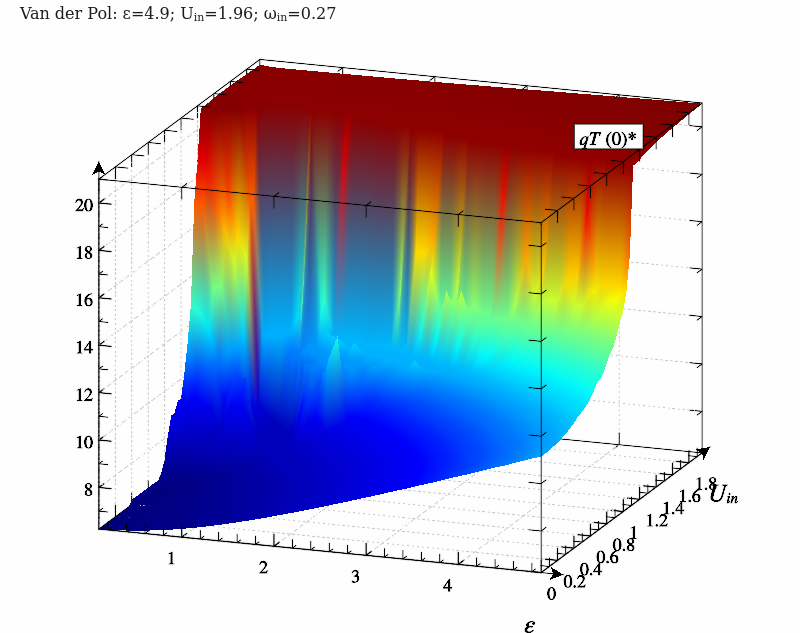
\includegraphics[width=0.49\textwidth]{p/cha/vdp/vdp_q_2d-p_qT_ome_0x27.png}
  \hfill
  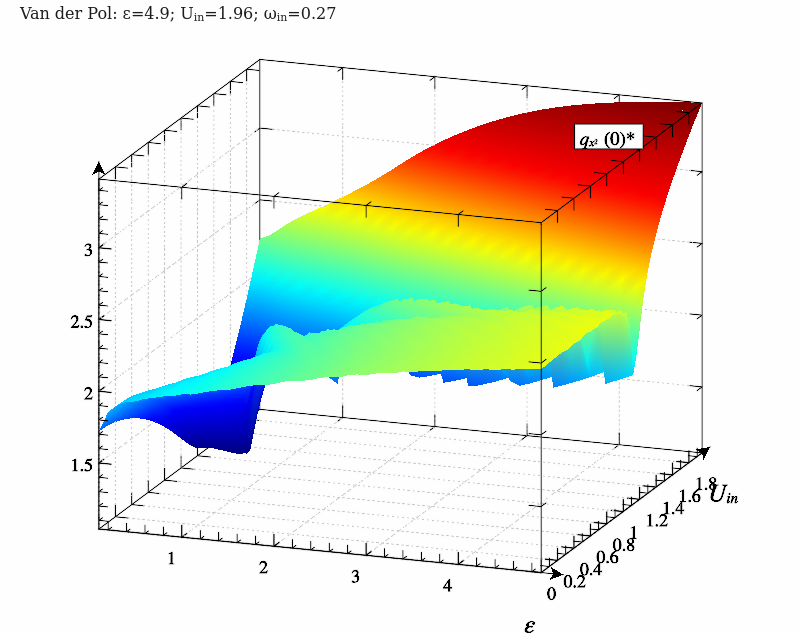
\includegraphics[width=0.49\textwidth]{p/cha/vdp/vdp_q_2d-p_qx2_ome_0x27.png}
\end{center}
  \caption{Залежності $q_T(\varepsilon,U_{in})$ та $q_{x^2}(\varepsilon,U_{in})$  при $\omega_{in}=0.27$}
\label{atu:f:vdp_q2_027}
\end{figure}

При високих значеннях
$ U_{in} $ відбувається захоплення частоти, графік залежності
$ q_T (\varepsilon, U_{in}) $ в цій області є плоску поверхню, що свідчить
про непридатність критерію в цих умовах. При малих значення
$ U_{in} $, навпаки, спостерігається досить близька до лінійної
залежність. У проміжку між двома цими областями можливості
ідентифікації з використанням даного критерію існують, але
обмежені. Критерій
$q_{x^2} $ при цих же умовах має дещо інші обмеження. Ідентифікація
утруднена в області ``яру'', який відповідає перехідному режиму
на попередньому графіку. Як в області низьких, так і в області
високих значень
$ U_{in} $ ідентифікація можлива.

На рис.~\ref{atu:f:vdp_q2_120} представлені поверхні критеріїв при
$ \omega_{in} = 1.2 $.

\begin{figure}[ht!]
\begin{center}
  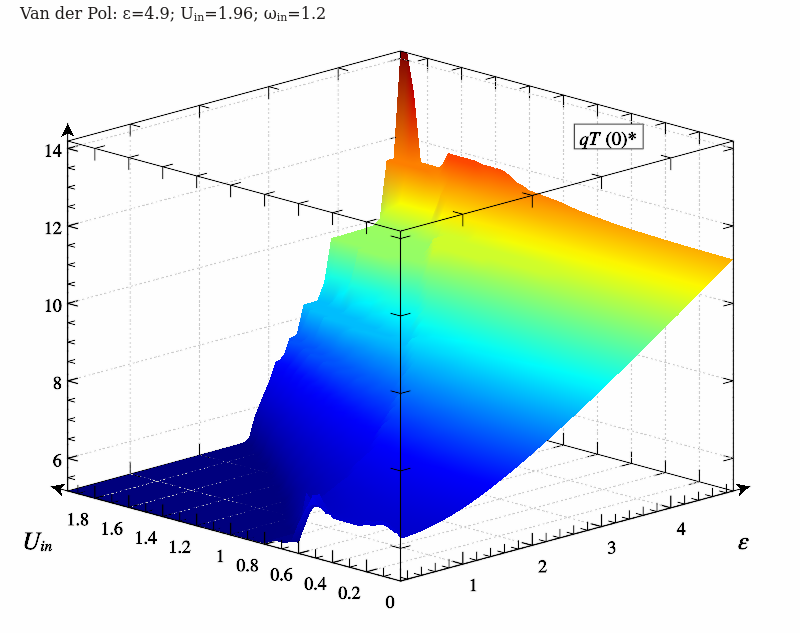
\includegraphics[width=0.49\textwidth]{p/cha/vdp/vdp_q_2d-p_qT_ome_1x20.png}
  \hfill
  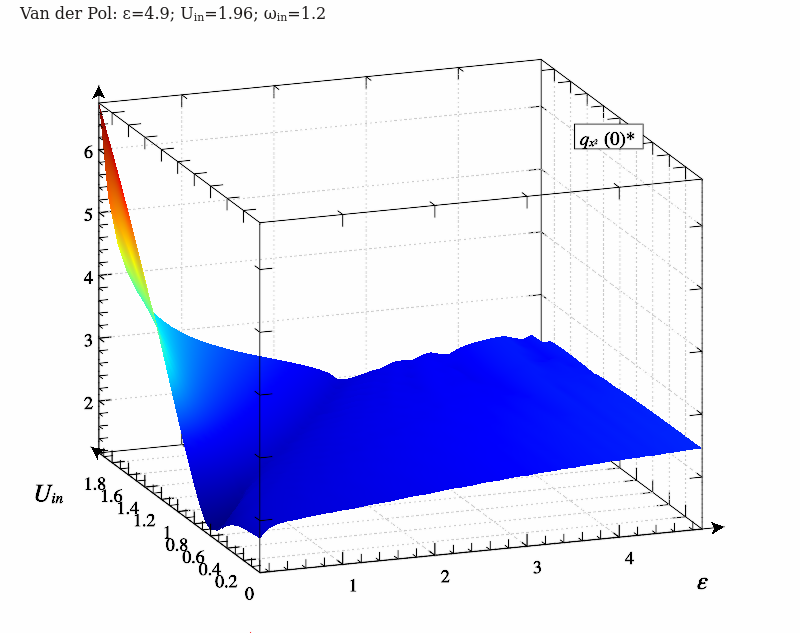
\includegraphics[width=0.49\textwidth]{p/cha/vdp/vdp_q_2d-p_qx2_ome_1x20.png}
\end{center}
  \caption{Залежності $q_T(\varepsilon,U_{in})$ та $q_{x^2}(\varepsilon,U_{in})$  при $\omega_{in}=1.2$}
\label{atu:f:vdp_q2_120}
\end{figure}

На залежності
$ q_T (\varepsilon, U_{in}) $ в цьому випадку також видно плоску ділянку,
що відповідає режиму захоплення частоти. Але більша частина
цієї залежності свідчить про те, що ідентифікація можлива,
і при цьому швидше за все буде спостерігатися збільшення
похибки ідентифікації через нерівномірність графіка. Навпаки,
залежність
$ q_T (\varepsilon, U_{in}) $ проявляє мультимодальний характер, що дозволяє
проводити ідентифікацію тільки у вузьких діапазонах.

Таким чином, встановлено, що жоден з розглянутих критеріїв не
забезпечує можливість ідентифікації при будь-яких значеннях
параметрів. Однак, найбільший діапазон працездатності
продемонстрував критерій
$q_{T}$. Він і буде використаний в подальших дослідженнях. При
цьому при постановці завдання будемо уникати режимів, на яких
відбувається захоплення частоти.

% }}}2

\subsection{Тестова задача ідентифікації для системи Ван-дер-Поля} % {{{2

При синтезу системи ідентифікації використовувалася група
методів ``ql3rlWvnAAW''. З урахуванням вибору критерію
$ q_{T} $ при постановці задачі ідентифікації параметри
вибиралися з урахуванням діапазону працездатності цього
критерію. Перша група значень параметрів:
$ U_{in} = 0.3 $,
$ \omega_{in} = 0.27 $,
$ \varepsilon \in [1, 4]$.

Розглянемо процес ідентифікації в квазістаціонарному випадку,
при повільної зміні параметра~(\ref{atu:eq:po_t_ramp}),
$ p_0 = 1 $,
$ U_p = 2 $. Динаміка агентів і різних способів завдання
$ p_\mathrm{id} $ представлена на рис.~\ref{atu:f:vdp_id1_ramp}.

\begin{figure}[ht!]
\begin{center}
  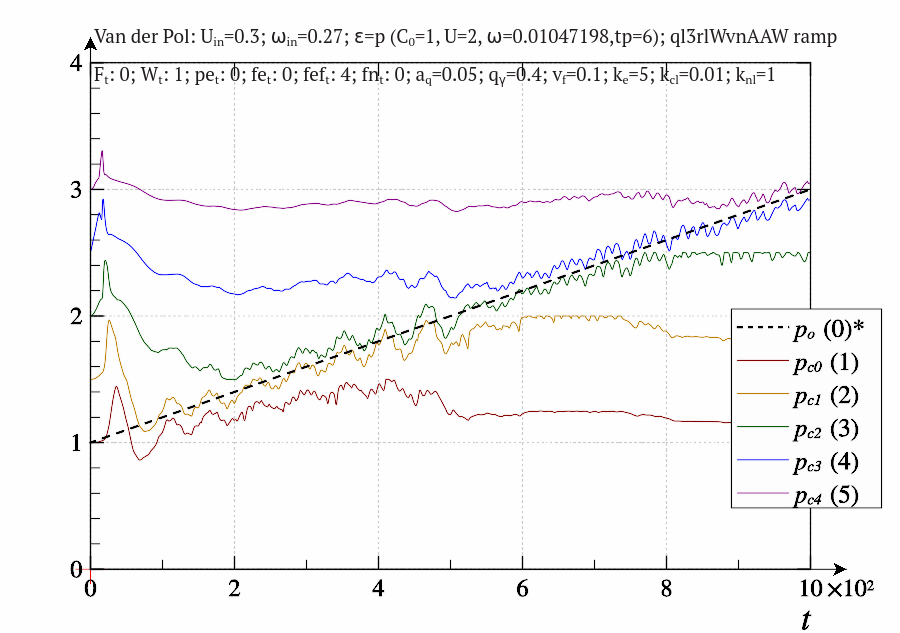
\includegraphics[width=0.49\textwidth]{p/cha/vdp/vdp_id-p_t_pi_ql3rlWvnAAW_ramp.png}
  \hfill
  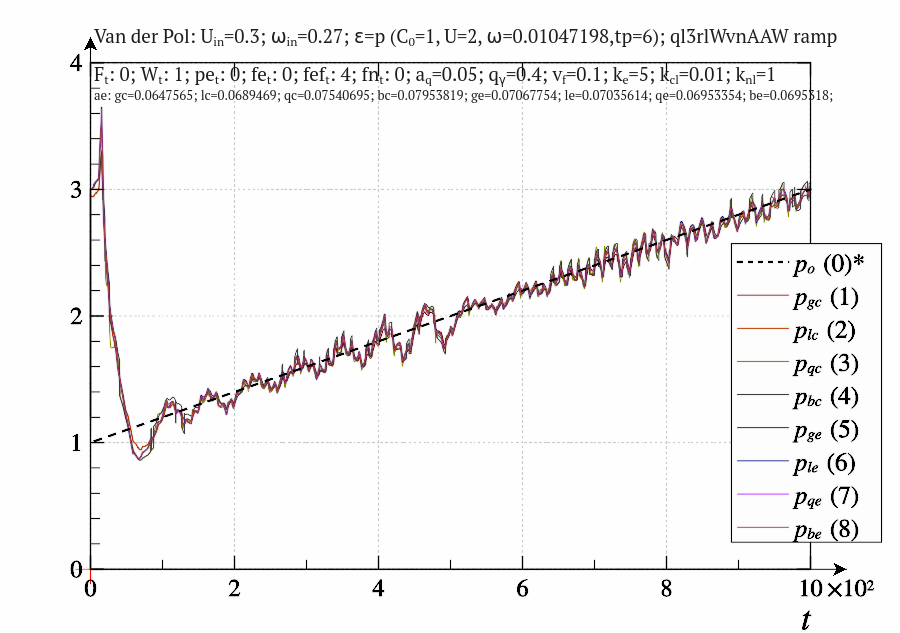
\includegraphics[width=0.49\textwidth]{p/cha/vdp/vdp_id-p_t_p_ql3rlWvnAAW_ramp.png}
\end{center}
\caption{Динаміка агентів і ідентифікованого значення для системи Ван-дер-Поля за умови (\ref{atu:eq:po_t_ramp})}
\label{atu:f:vdp_id1_ramp}
\end{figure}

За винятком початкової ділянки, на якої відбувається
стабілізація стану самої системи ідентифікації, агенти
демонструють коректну поведінку, супроводжуючи значення параметра
$ \varepsilon $, яке повільно змінюється.
Як наслідок, всі методи визначення
$ p_\mathrm{id} $ дозволяють досить точно провести
ідентифікацію. Невеликі коливання обумовлені тим, що насправді
система не в повній мірі може бути названа квазістаціонарною,
через великий часу усереднення критерію. Ділянок, на яких
порушувався б процес ідентифікації, або ж істотно зросла
похибка, не спостерігається.

Розглянемо динамку процесу ідентифікації (рис.~\ref{atu:f:vdp_id1_sign})
при умовах (\ref{atu:eq:po_t_sign}),
$ p_0 = 2 $,
$ U_p = 0.8 $,
$ \omega_{in} = 0.01047 $.

\begin{figure}[ht!]
\begin{center}
  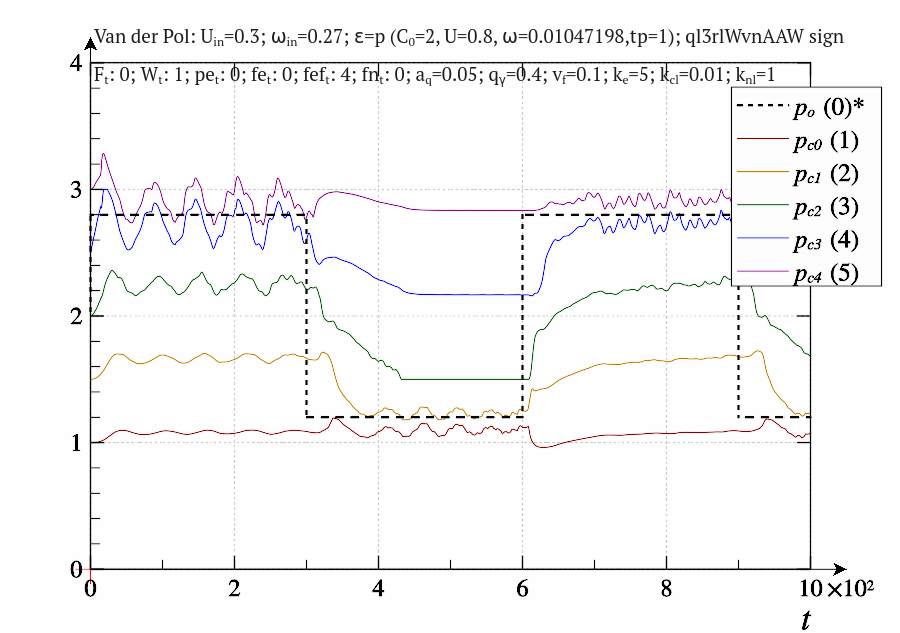
\includegraphics[width=0.49\textwidth]{p/cha/vdp/vdp_id-p_t_pi_ql3rlWvnAAW_sign.png}
  \hfill
  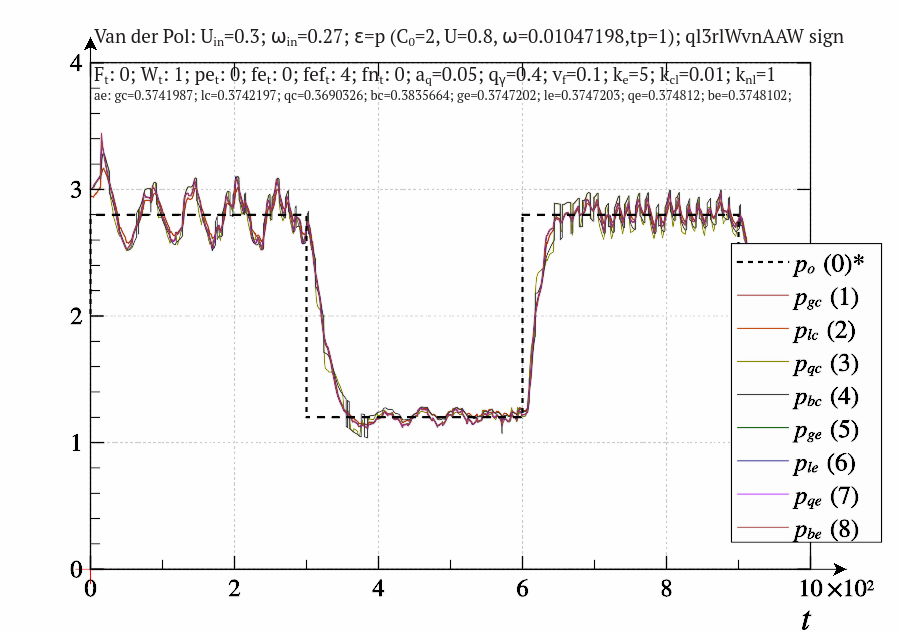
\includegraphics[width=0.49\textwidth]{p/cha/vdp/vdp_id-p_t_p_ql3rlWvnAAW_sign.png}
\end{center}
\caption{Динаміка агентів і ідентифікованого значення для системи Ван-дер-Поля за умови (\ref{atu:eq:po_t_sign})}
\label{atu:f:vdp_id1_sign}
\end{figure}

Як вже спостерігалося, усі методи визначення
$ p_\mathrm{id} $ на рівні координатора пошуку дають схожі
результати. Слід зазначити помітні коливання на першій половині
періоду зміни параметра, в порівнянні з третім. Надмірні
коливанням на початковому етапі можна зменшити шляхом
попередньої настройки елементів усереднення критерію. Однак,
для такого налаштування необхідна додаткова інформація, яка
невідома a priori.

На рис.~\ref{atu:f:vdp_id1_sin} представлені аналогічні результати, але
в разі плавної зміни параметра~(\ref{atu:eq:po_t_sin}).

\begin{figure}[ht!]
\begin{center}
  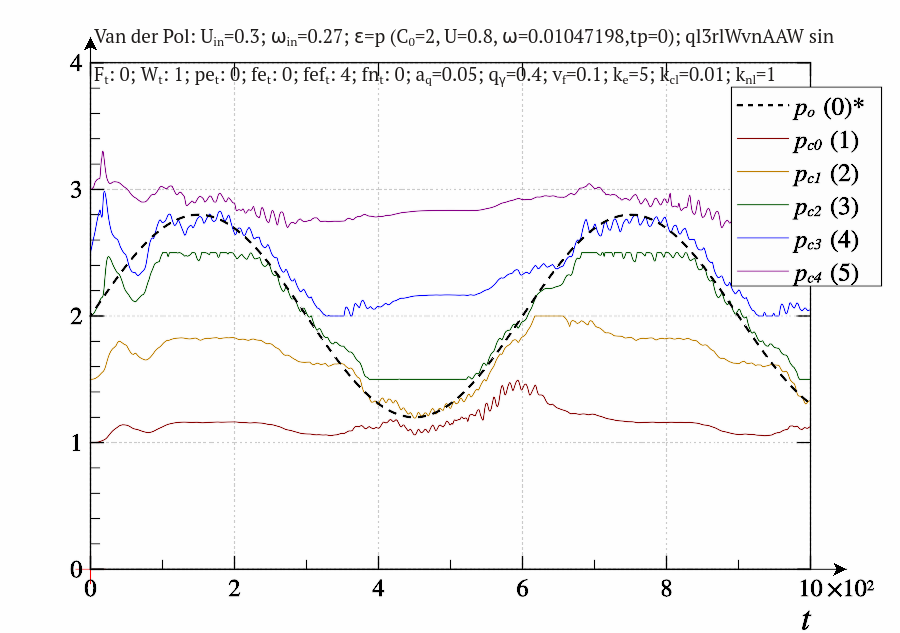
\includegraphics[width=0.49\textwidth]{p/cha/vdp/vdp_id-p_t_pi_ql3rlWvnAAW_sin.png}
  \hfill
  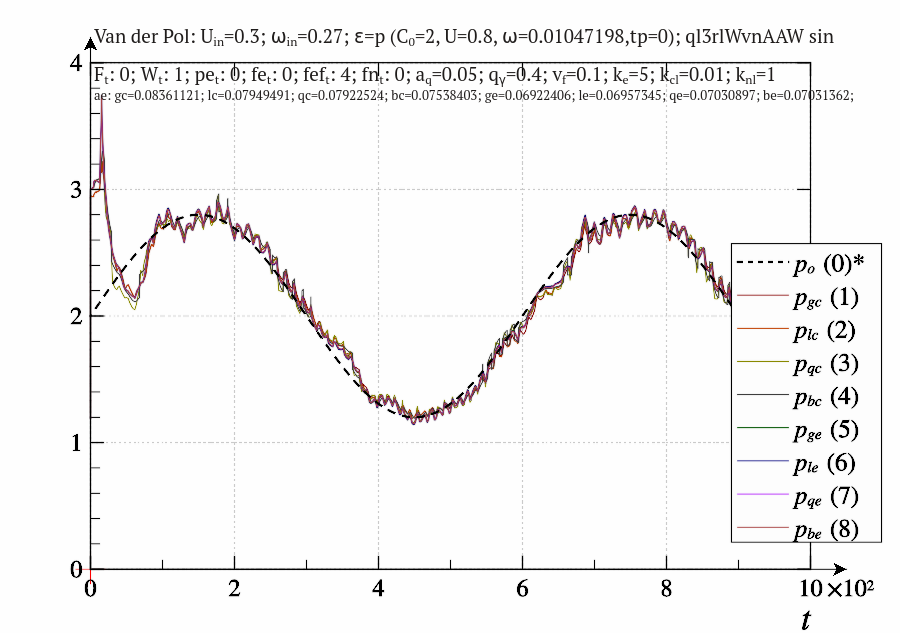
\includegraphics[width=0.49\textwidth]{p/cha/vdp/vdp_id-p_t_p_ql3rlWvnAAW_sin.png}
\end{center}
\caption{Динаміка агентів і ідентифікованого значення для системи Ван-дер-Поля за умови (\ref{atu:eq:po_t_sin})}
\label{atu:f:vdp_id1_sin}
\end{figure}

Помилка ідентифікації в цьому випадку істотно менше, також
зберігаються коливання на початковому етапі.

% }}}2


\subsection{Вплив параметрів системи ідентифікації на похибку ідентифікації для системи Ван-дер-Поля} % {{{2

При ідентифікації системи Ван-дер-Поля з використанням критерію
$q_T$ вплив параметра
$a_q$ представляє особливий інтерес, зважаючи на наявність двох
рівнів усереднення. Залежності усереднених помилок ідентифікації
від цього параметра представлені на рис.~\ref{atu:f:vdp_e_a_q}.

\begin{figure}[ht!]
\begin{center}
  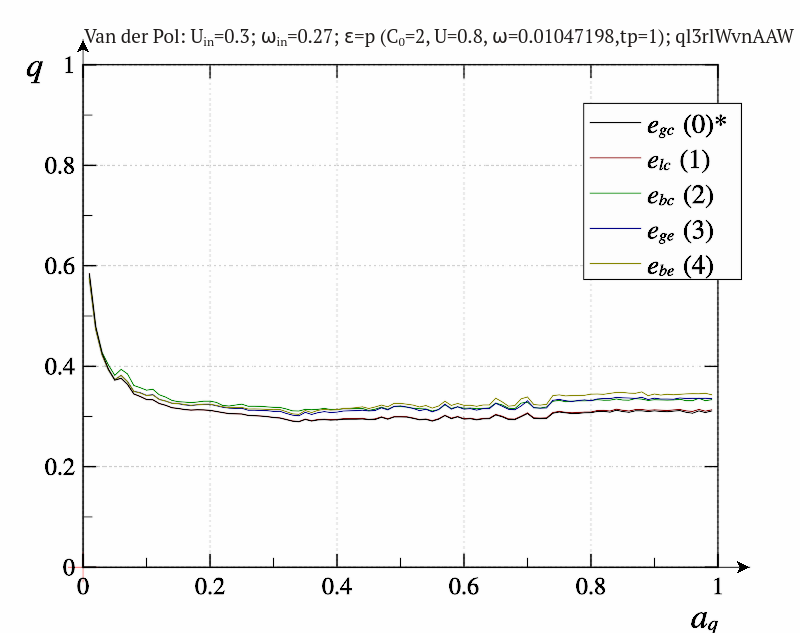
\includegraphics[width=0.49\textwidth]{p/cha/vdp/vdp_id-p_a_q_sign.png}
  \hfill
  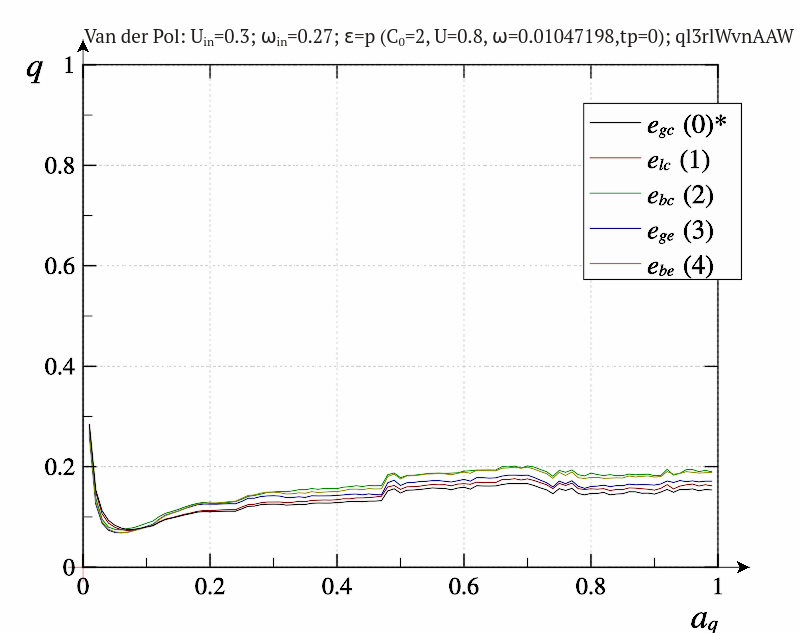
\includegraphics[width=0.49\textwidth]{p/cha/vdp/vdp_id-p_a_q_sin.png}
\end{center}
  \caption{Залежності $\bar{e}(a_q)$ для системи Ван-дер-Поля}
\label{atu:f:vdp_e_a_q}
\end{figure}

Виходячи з характерних значень ``періоду'' можна було б очікувати
зміну характеру цих залежностей при
$ a_q \approx 0.1 $. Однак, ніяких істотних змін на графіках не
виявлено. Сам вигляд цих залежностей практично нічим, крім
масштабу, не відрізняється від таких для вже розглянутих
систем. Таким чином отримала підтвердження теза про необхідність
додаткового усереднення на цьому етапі.

Розглянемо вплив ще одного параметра системи ідентифікації ---
$ q_\gamma $. Відповідні залежності наведені на рис.~\ref{atu:f:vdp_e_q_gamma}.

\begin{figure}[ht!]
\begin{center}
  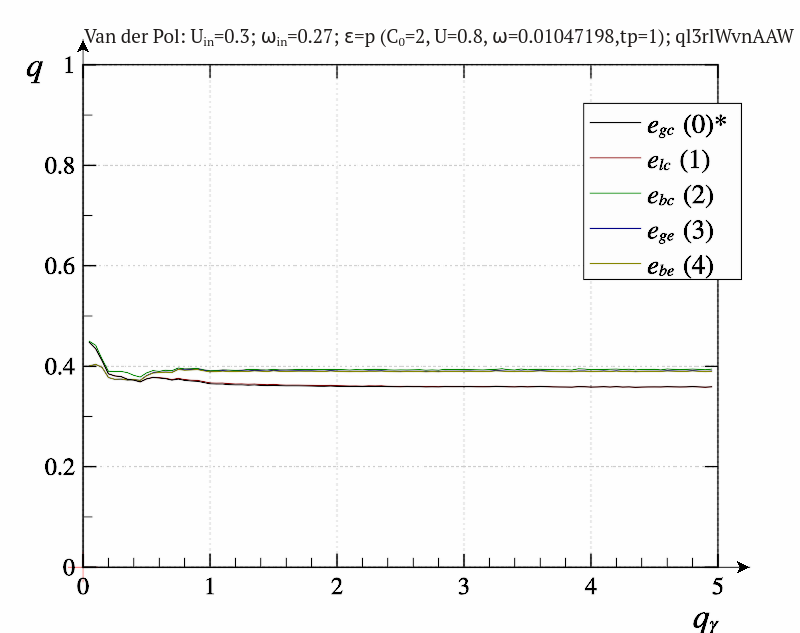
\includegraphics[width=0.49\textwidth]{p/cha/vdp/vdp_id-p_q_gamma_sign.png}
  \hfill
  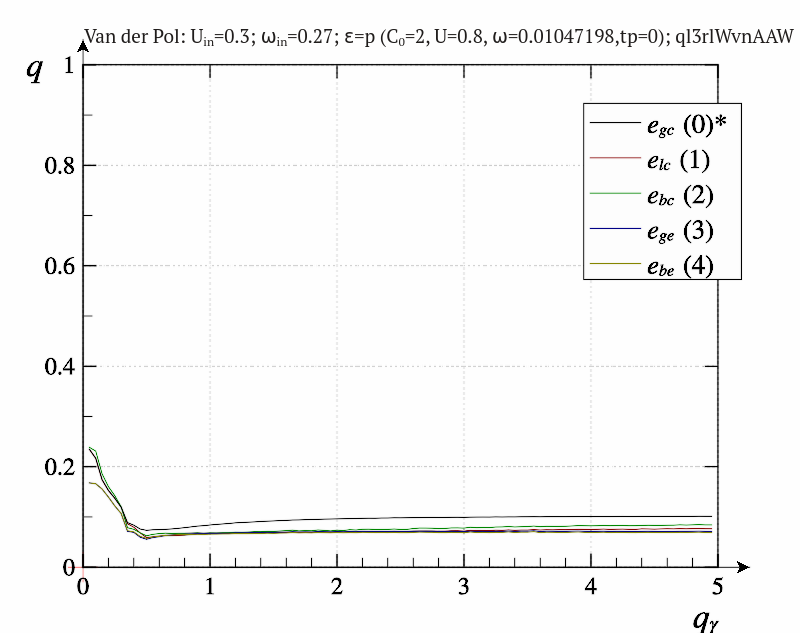
\includegraphics[width=0.49\textwidth]{p/cha/vdp/vdp_id-p_q_gamma_sin.png}
\end{center}
  \caption{Залежності $\bar{e}(q_\gamma)$ для системи Ван-дер-Поля}
\label{atu:f:vdp_e_q_gamma}
\end{figure}

Використовувана група методів ``ql3rlWvnAAW'' характеризується
працездатністю для широкого діапазону величини
$ q_\gamma $, за винятком області надмірної чутливості, у
якої пошук все ж можливий, але його діапазон обмежується
малим околом агентів. Представлені графіки повністю це
підтверджують. Застосування різних методів визначення
$p_\mathrm{id} $ по різному себе проявляє в області заниженої
чутливості, але ця різниця мала.


Залежності
$ \bar{e} (v_f) $ отримані при ідентифікації системи Ван-дер-Поля
(рис.~\ref{atu:f:vdp_e_v_f}), демонструють істотну різницю при різних
способах завдання нестаціонарності параметра.

\begin{figure}[ht!]
\begin{center}
  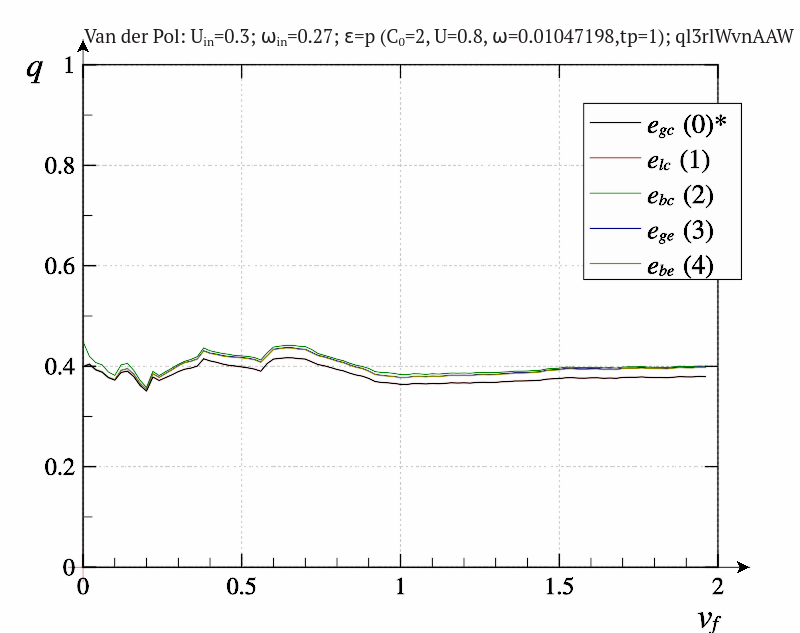
\includegraphics[width=0.49\textwidth]{p/cha/vdp/vdp_id-p_v_f_sign.png}
  \hfill
  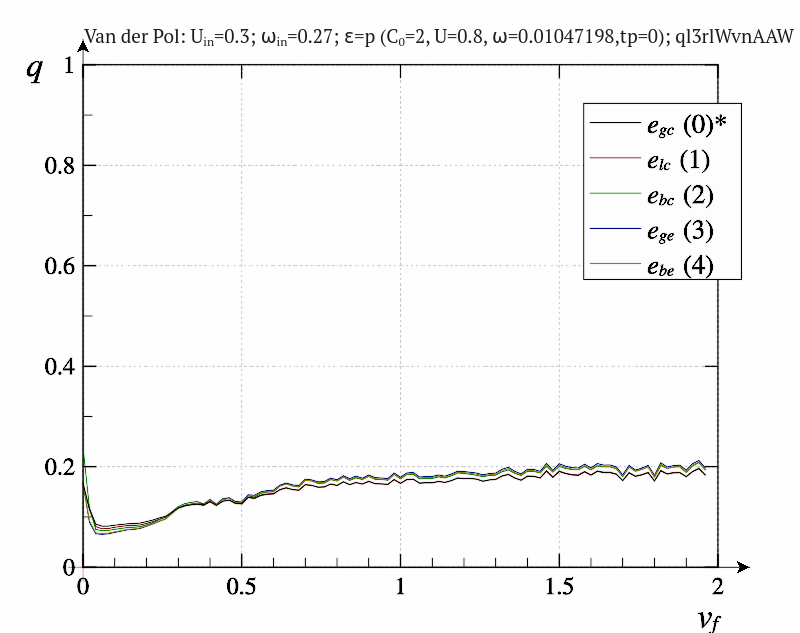
\includegraphics[width=0.49\textwidth]{p/cha/vdp/vdp_id-p_v_f_sin.png}
\end{center}
  \caption{Залежності $\bar{e}(v_f)$ для системи Ван-дер-Поля}
\label{atu:f:vdp_e_v_f}
\end{figure}

Якщо в динаміці ідентифікованого параметра немає різких змін
(правий графік), то залежності мають класичний вигляд, тобто існує таке
значення $ v_f $, при якому спостерігається мінімум похибки. У тому
ж випадку, коли залежність являє собою залежність з
розривами (\ref{atu:eq:po_t_sign}), то вплив стає слабким
і неоднозначним. Це пов'язано з тим, що перебудова положень
агентів хоч і відбувається, але не призводить до зменшення
похибки з огляду на те, що час реакції критерію стає одного
порядку з часом реакції на зміну параметра.


Вплив коефіцієнта
$ k_e $ (рис.~\ref{atu:f:vdp_e_k_e}) для даної системи також істотно залежить
від динаміки параметра, і з тієї ж причини. Якщо динаміка
параметра задана як (\ref{atu:eq:po_t_sin}), то існує екстремум, що
відповідає оптимальному розподілу агентів. При стрибкоподібних
змінах параметра екстремум практично непомітний на загальному рівні.

\begin{figure}[ht!]
\begin{center}
  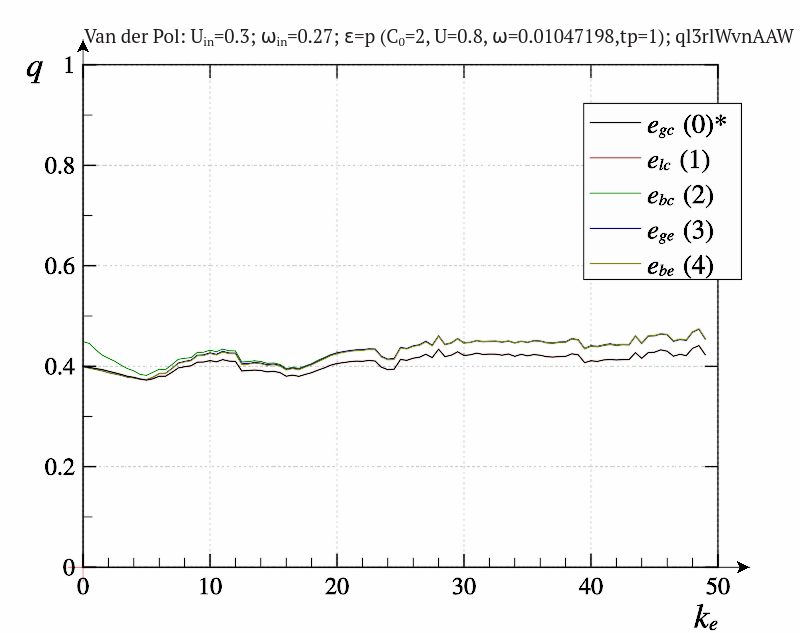
\includegraphics[width=0.49\textwidth]{p/cha/vdp/vdp_id-p_k_e_sign.png}
  \hfill
  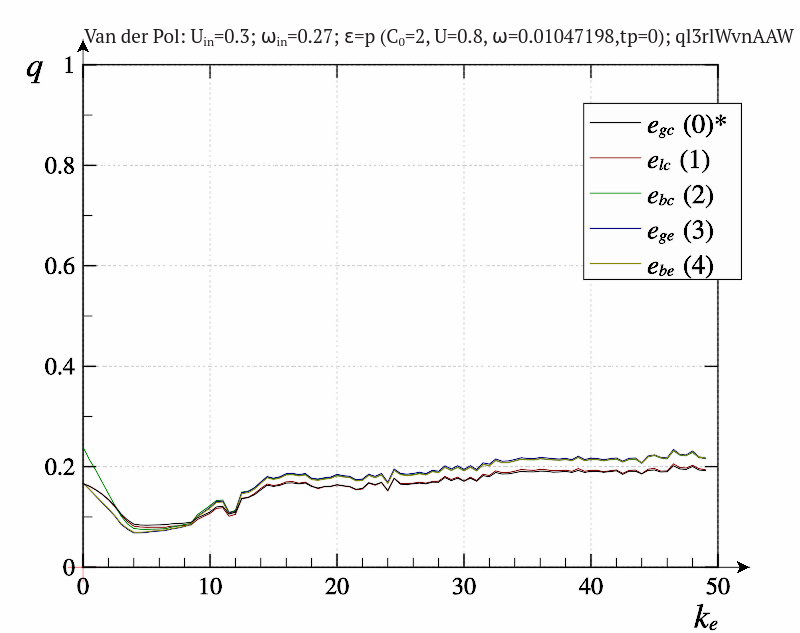
\includegraphics[width=0.49\textwidth]{p/cha/vdp/vdp_id-p_k_e_sin.png}
\end{center}
  \caption{Залежності $\bar{e}(k_e)$ для системи Ван-дер-Поля}
\label{atu:f:vdp_e_k_e}
\end{figure}

Вплив параметра
$ k_{nl} $ (рис.~\ref{atu:f:vdp_e_k_nl}) відображає властивості множини агентів
як ансамблю. На відміну від двох попередніх залежностей, мінімум
похибки ідентифікації спостерігається для двох способів
визначення динаміки параметрів, тобто коректна взаємодія
між агентами необхідна для отримання результату навіть в тих
випадках, коли власне переміщення агентів не виправдано.

\begin{figure}[ht!]
\begin{center}
  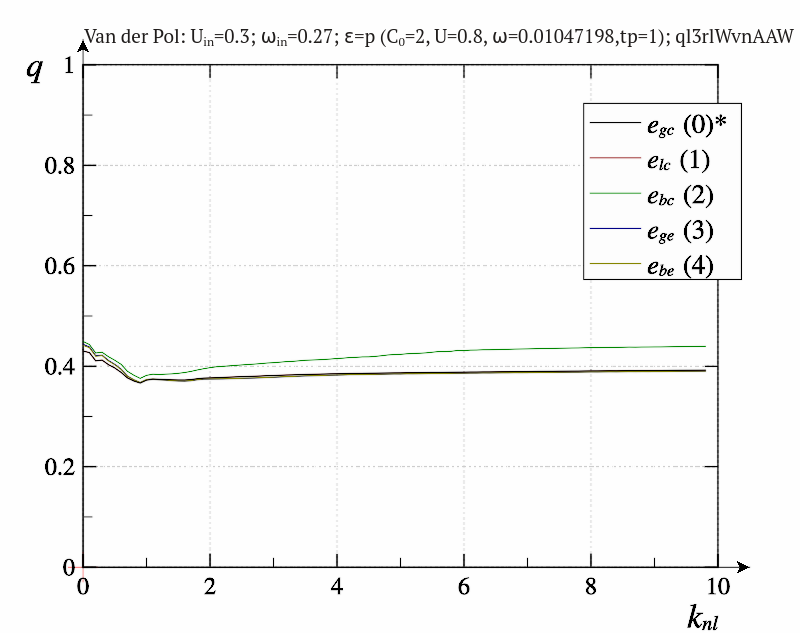
\includegraphics[width=0.49\textwidth]{p/cha/vdp/vdp_id-p_k_nl_sign.png}
  \hfill
  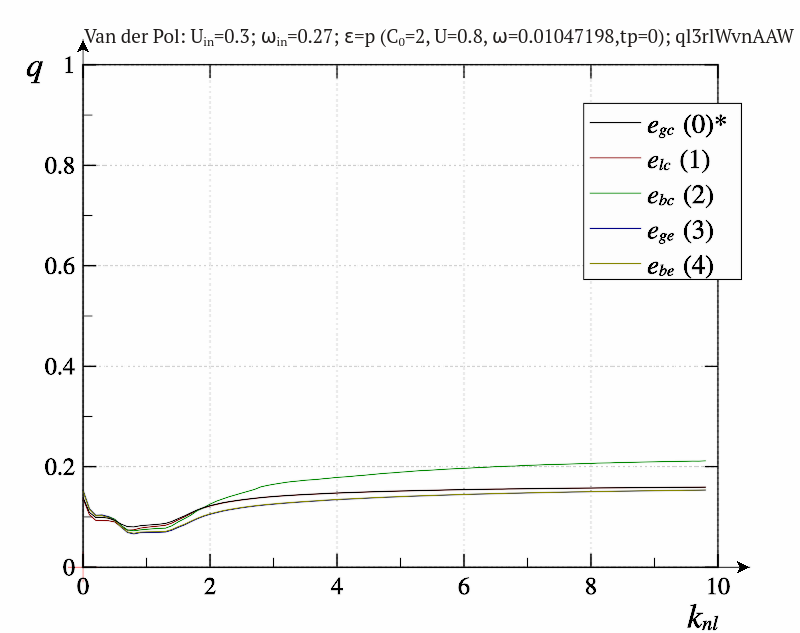
\includegraphics[width=0.49\textwidth]{p/cha/vdp/vdp_id-p_k_nl_sin.png}
\end{center}
  \caption{Залежності $\bar{e}(k_{nl})$ для системи Ван-дер-Поля}
\label{atu:f:vdp_e_k_nl}
\end{figure}

Як і в попередньому випадку, штучні обмеження на переміщення
агентів практично нівелює вплив коефіцієнта
$ k_{cl} $ (рис.~\ref{atu:f:vdp_e_k_cl}). У цих умовах силу
$ f_c $ має сенс взагалі не визначати.

\begin{figure}[ht!]
\begin{center}
  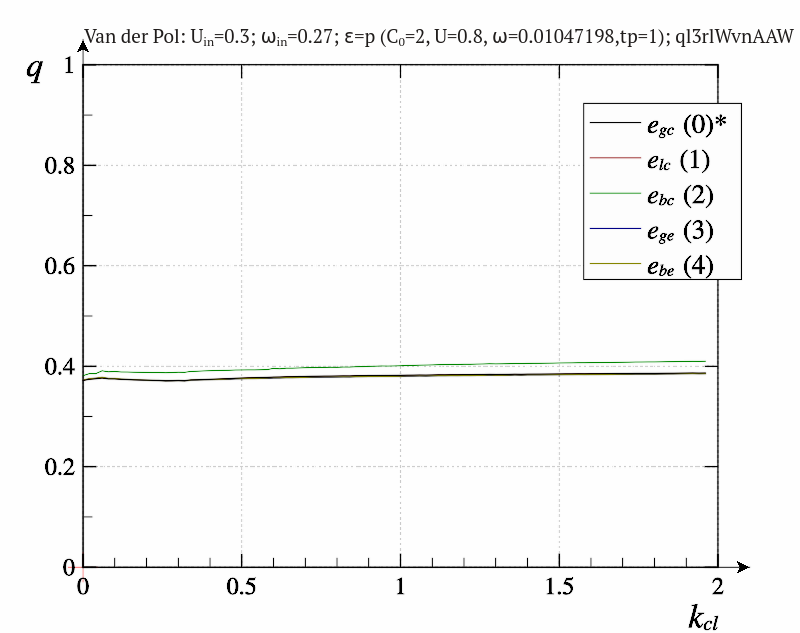
\includegraphics[width=0.49\textwidth]{p/cha/vdp/vdp_id-p_k_cl_sign.png}
  \hfill
  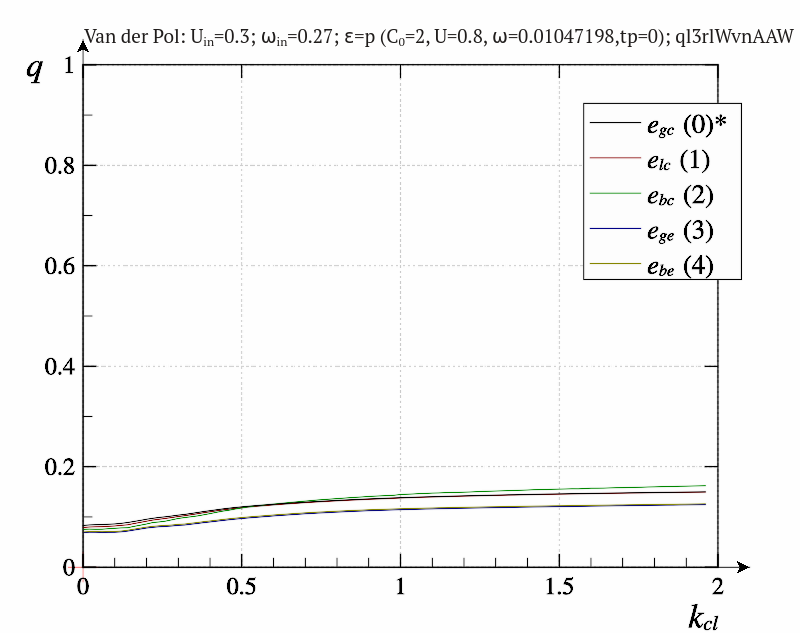
\includegraphics[width=0.49\textwidth]{p/cha/vdp/vdp_id-p_k_cl_sin.png}
\end{center}
  \caption{Залежності $\bar{e}(k_{cl})$ для системи Ван-дер-Поля}
\label{atu:f:vdp_e_k_cl}
\end{figure}

На рис.~\ref{atu:f:vdp_e_varepsilon_2} представлена залежність похибки
ідентифікації від величини самого параметра
$ \varepsilon $ в умовах, коли постійно чергуються хаотичні і
складно-періодичні режими. У цих умовах похибка ідентифікації
зростає, але сама система ідентифікації залишається
працездатною.


\begin{figure}[ht!]
\begin{center}
  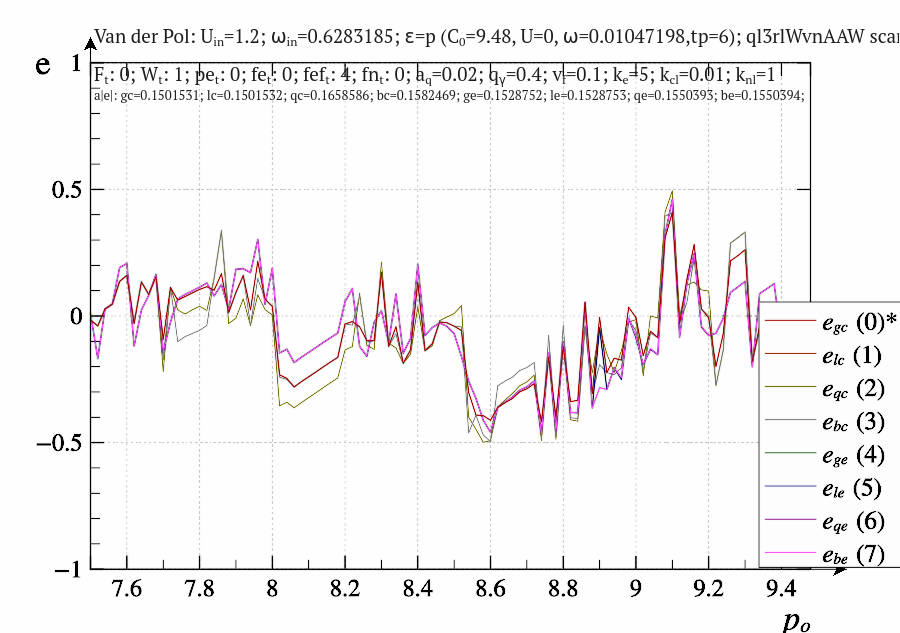
\includegraphics[width=0.60\textwidth]{p/cha/vdp/vdp_id2-p_p_e_ql3rlWvnAAW_scan.png}
\end{center}
  \caption{Залежності $\bar{e}(\varepsilon)$ для системи Ван-дер-Поля за умов чергування режимів коливань}
\label{atu:f:vdp_e_varepsilon_2}
\end{figure}

% }}}2

\subsection{Висновки}%{{{2

Результати моделювання процесів ідентифікації параметра ``$\varepsilon$''
системи Ван-дер-Поля дозволяють зробити наступні
висновки:

\begin{itemize}

  \item
    Найбільший діапазон зразковості для цієї системи демонструє
    критерій $ q_T $ з наступним усередненням.

  \item
    Не виявлено критерію, який би був працездатний у всій області
    визначення параметрів, в зв'язку з різноманітністю динаміки,
    яку проявляє система.

  \item
    Група методів ql3rlWvnAAW показала свою хорошу працездатність,
    навіть в умовах чергування режимів коливань.

  \item
    Параметри самої системи ідентифікації можуть змінюватися
    в досить широких межах без істотного збільшення похибки
    ідентифікації.

\end{itemize}

% }}}2



% }}}1

% vim: fdm=marker foldlevel=1 foldignore="%#" fdc=4 ft=tex
